\documentclass[11pt,a4paper]{article}
\usepackage[T1]{fontenc}
\usepackage[margin=2.3cm]{geometry}
\usepackage{amsmath,amssymb}
\usepackage{graphicx}
\usepackage[dvipsnames]{xcolor}
\usepackage{enumitem}
\usepackage[colorlinks=true,linkcolor=blue,urlcolor=blue]{hyperref}
\setlength{\parskip}{0.6em}
\setlength{\parindent}{0pt}
\begin{document}

\begin{center}{\LARGE\bfseries openhydraulics}\\[0.4em]{\large Lift a car with one hand using Pascal's law, in three sessions.}\\[0.2em]\small PAN IIT OSS explainer \textbullet{} higher secondary to diploma / undergraduate (levels 4-5)\end{center}

\section*{Why this exists}
A hydraulic jack lets one hand lift a car. This explainer shows the physics behind it: pressure, Pascal's law, the trade between force and distance, and a simulation of a lift with a pump, a relief valve and leaking oil, using only simple equations so you can build it yourself.

\section*{The end goal}
Lift a car with a small force using Pascal's law. The end goal is to lift a car with a small force using Pascal's law. The same ideas drive garage lifts, brakes, excavators and aircraft flaps; real machines need certified design, safety locks and professional engineering.

\section*{How the three sessions build up}
\begin{enumerate}[nosep]
\item \textbf{Session 1: A small push, a big lift} (Level 1, conceptual interactive model, 60 min).
\item \textbf{Session 2: The equations of a hydraulic jack} (Level 2, mathematical engineering model, 75 min).
\item \textbf{Session 3: Simulate a hydraulic lift} (Level 3, simulation and validation, 90 min).
\end{enumerate}

\section{Session 1: A small push, a big lift}

\subsection*{A. Real-world problem}
A garage jack lifts a whole car when you pump a handle with one hand. A car weighs about 12 000 newtons, far more than you can lift, so where does the extra force come from? Nothing is magic: the liquid in the jack passes the same pressure from a small piston to a big piston, and a big piston turns that pressure into a bigger force. What do we pay for the gain?

\subsection*{B. Concept and theory}
Pressure is force spread over an area: p = F / A. Pascal's law says that in a liquid at rest, a pressure added at one place is felt equally in all directions and at every point of the liquid. In a two-piston machine the same pressure p acts on both pistons, so F1 / A1 = F2 / A2 and the force on the big piston is F2 = F1 (A2 / A1). The area of a round piston is A = pi d\textasciicircum{}2 / 4, so doubling the diameter makes the area, and the force, four times bigger. The liquid cannot be squashed, so the volume that leaves the small cylinder enters the big one: A1 s1 = A2 s2. The big piston therefore moves only s2 = s1 (A1 / A2): force multiplies, distance divides.

\begin{itemize}[nosep]
\item p: pressure in the liquid (Pa (N/m\textasciicircum{}2))
\item F1, F2: force on the small and the big piston (N)
\item A1, A2: area of the small and the big piston (m\textasciicircum{}2)
\item d1, d2: diameter of the small and the big piston (m)
\item s1, s2: distance moved by the small and the big piston (m)
\end{itemize}

\begin{equation*}
p=\frac{F}{A},\qquad A=\frac{\pi d^{2}}{4}
\end{equation*}

\begin{equation*}
\frac{F_1}{A_1}=\frac{F_2}{A_2}\ \Rightarrow\ F_2=F_1\,\frac{A_2}{A_1}=F_1\left(\frac{d_2}{d_1}\right)^{2}
\end{equation*}

\begin{equation*}
A_1 s_1=A_2 s_2\ \Rightarrow\ s_2=s_1\,\frac{A_1}{A_2}
\end{equation*}

\begin{center}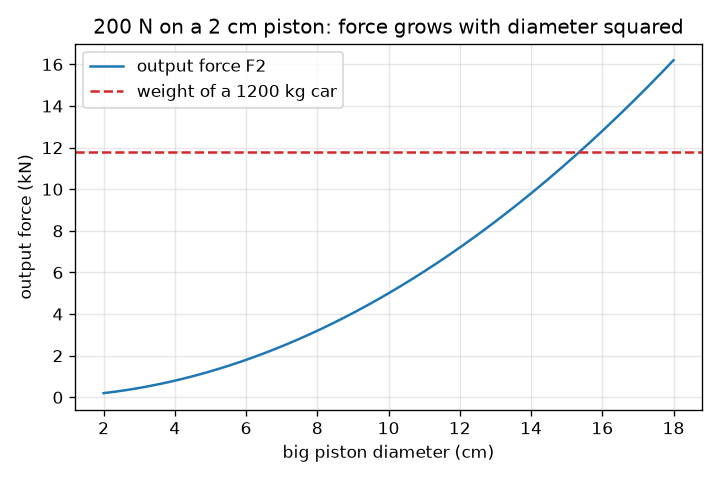
\includegraphics[width=0.85\linewidth]{figures/s01_force_vs_diameter.png}\\\small Output force against big piston diameter for a 200 N push on a 2 cm piston, with the weight of a 1200 kg car.\end{center}

\subsection*{E. Worked example}
A 200 N push acts on a small piston of diameter 2 cm. The big piston has diameter 6 cm. Find the pressure, the force on the big piston, the multiplier, and how far the big piston moves when the small piston moves 5 cm. Check that the work is the same on both sides.
\begin{enumerate}[nosep]
\item Small piston area: A1 = pi * 0.02\textasciicircum{}2 / 4 = 3.142e-4 m\textasciicircum{}2.
\item Pressure: p = F1 / A1 = 200 / 3.142e-4 = 636 600 Pa = 636.6 kPa (about 6.4 times atmospheric pressure).
\item Multiplier = (d2 / d1)\textasciicircum{}2 = (6 / 2)\textasciicircum{}2 = 9, so F2 = 9 * 200 = 1800 N.
\item Distance: s2 = s1 / 9 = 50 mm / 9 = 5.6 mm.
\item Work in: 200 N * 0.05 m = 10 J. Work out: 1800 N * 0.00556 m = 10 J. They agree.
\end{enumerate}
\textbf{Answer.} p = 636.6 kPa, F2 = 1800 N, multiplier 9, the big piston moves 5.6 mm, and the work in and out is 10 J.

\subsection*{F. Questions}
\begin{enumerate}[nosep]
\item \textbf{Conceptual.} A hydraulic jack gives a force of 1800 N from a push of 200 N. Does this break the law that energy cannot be created? Explain with the distances moved.
\item \textbf{Numerical.} A force of 300 N pushes a small piston of diameter 2.5 cm. The big piston has diameter 10 cm. Find the pressure in kPa and the force on the big piston.
\item \textbf{Graph and simulation interpretation.} In the force graph (200 N on a 2 cm piston), at which big piston diameter does the output force first equal the weight of a 1200 kg car, and what does the curve tell you about doubling the diameter?
\item \textbf{Design and optimisation challenge.} Design: you can push with 150 N on a pump piston of diameter 1.5 cm and must lift a 500 kg load (4905 N). Choose a big piston diameter, and say how far you must push to raise the load 1 cm.
\end{enumerate}

\section{Session 2: The equations of a hydraulic jack}

\subsection*{A. Real-world problem}
A workshop wants to lift a 1200 kg car by pushing a lever with no more than 200 N. How wide must the pistons be? How long a lever do we need? And how many pumps of the handle does each centimetre of lift cost? Answering needs the equations of Session 1 with careful units, and a first look at the pressure that the weight of a liquid itself makes.

\subsection*{B. Concept and theory}
Pressure is p = F / A and is measured in pascals (1 Pa = 1 N/m\textasciicircum{}2); we also use kPa (1000 Pa) and bar (100 000 Pa, close to one atmosphere, 101 325 Pa). Pascal's law gives F2 = F1 (A2 / A1), and the mechanical advantage is MA = F2 / F1 = A2 / A1. For an ideal jack the liquid volume moved is equal on both sides, A1 d1 = A2 d2, so F1 d1 = F2 d2: the work put in equals the work got out. Separately, a liquid at rest has a pressure that grows with depth h because of its own weight: p = rho g h (gauge pressure). In an open tank the absolute pressure is p\_atm + rho g h. A lever of ratio r (handle length divided by the distance from the pivot to the pump piston) multiplies the hand force, F1 = r F\_hand, while the handle moves r times as far as the pump piston. The car must satisfy F2 \textgreater{}= m g, so A2 \textgreater{}= A1 m g / F1. One pump stroke s1 raises the car by s1 / MA, so the number of pumps per centimetre is 0.01 m / (s1 / MA).

\begin{itemize}[nosep]
\item p: pressure (Pa, kPa or bar)
\item F, F1, F2: force (hand lever output, pump piston, big piston) (N)
\item A1, A2: pump piston and big piston area (m\textasciicircum{}2)
\item MA: mechanical advantage A2 / A1 (no unit)
\item rho: liquid density (oil 870, water 1000) (kg/m\textasciicircum{}3)
\item g: gravity, 9.81 (m/s\textasciicircum{}2)
\item h: depth below the surface (m)
\item r: lever ratio (no unit)
\item s1: pump piston stroke (m)
\item m: mass of the car (kg)
\end{itemize}

\begin{equation*}
p=\frac{F}{A},\qquad 1\ \mathrm{bar}=10^{5}\ \mathrm{Pa}
\end{equation*}

\begin{equation*}
F_2=F_1\frac{A_2}{A_1},\qquad \mathrm{MA}=\frac{A_2}{A_1},\qquad F_1 d_1=F_2 d_2
\end{equation*}

\begin{equation*}
p=\rho g h,\qquad p_{\mathrm{abs}}=p_{\mathrm{atm}}+\rho g h
\end{equation*}

\begin{equation*}
F_1=r F_{\mathrm{hand}},\qquad d_{2,\min}=d_1\sqrt{\frac{m g}{F_1}}
\end{equation*}

\begin{equation*}
\text{pumps per cm}=\frac{0.01\ \mathrm{m}}{s_1/\mathrm{MA}}
\end{equation*}

\begin{center}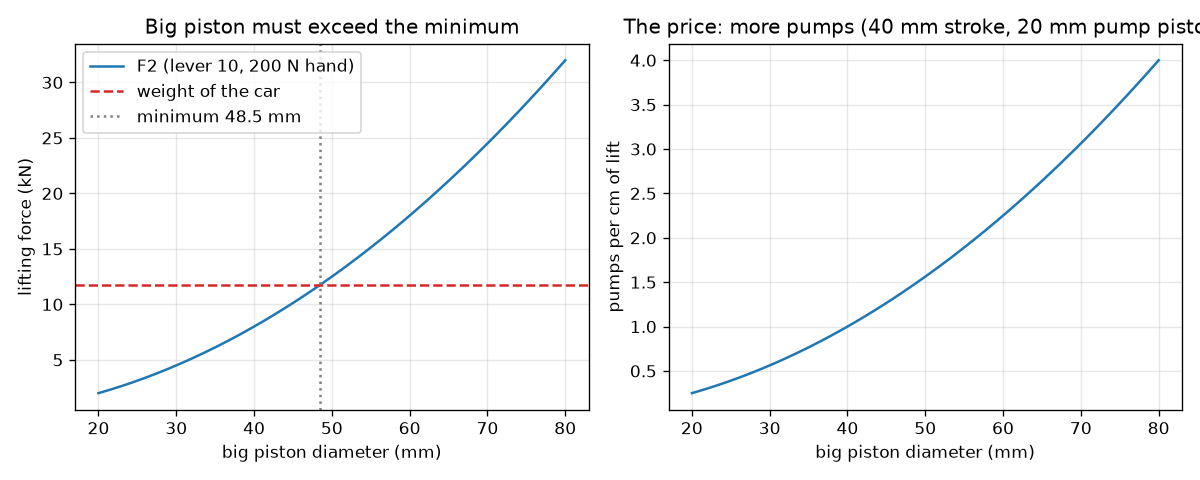
\includegraphics[width=0.85\linewidth]{figures/s02_design_curves.png}\\\small Design curves: force and pumps per centimetre against big piston diameter.\end{center}

\subsection*{E. Worked example}
Lift a 1200 kg car with a hand push of 200 N, a lever of ratio 10, a pump piston of 20 mm and a stroke of 40 mm. Find the smallest big piston, then check the choice of 50 mm: the pressure, the mechanical advantage, the lifting force, the lift per stroke, the number of pumps per centimetre and the work balance.
\begin{enumerate}[nosep]
\item Weight W = m g = 1200 * 9.81 = 11 772 N. Force on the pump piston F1 = 10 * 200 = 2000 N.
\item Smallest big piston: d2 = d1 sqrt(W / F1) = 20 mm * sqrt(11 772 / 2000) = 20 * 2.426 = 48.5 mm. Choose the next convenient size, 50 mm.
\item Areas: A1 = pi * 0.020\textasciicircum{}2 / 4 = 3.142e-4 m\textasciicircum{}2 and A2 = pi * 0.050\textasciicircum{}2 / 4 = 1.963e-3 m\textasciicircum{}2, so MA = 6.25.
\item Pressure p = F1 / A1 = 2000 / 3.142e-4 = 6.37 MPa = 63.7 bar. Force F2 = 6.25 * 2000 = 12 500 N, which is above 11 772 N (6 percent margin).
\item Lift per stroke = 40 mm / 6.25 = 6.4 mm, so pumps per cm = 10 mm / 6.4 mm = 1.56. The handle moves 10 * 40 = 400 mm per stroke.
\item Work balance: F1 * 0.040 m = 80 J and F2 * 0.0064 m = 80 J. They agree.
\end{enumerate}
\textbf{Answer.} Minimum big piston 48.5 mm; with 50 mm: MA 6.25, F2 = 12 500 N, p = 63.7 bar, 6.4 mm lift per stroke, 1.56 pumps per cm, 80 J of work per stroke in and out.

\subsection*{F. Questions}
\begin{enumerate}[nosep]
\item \textbf{Conceptual.} Why can we ignore rho g h inside the jack, but not when we design a dam or a diving bell?
\item \textbf{Numerical.} Find the gauge pressure and the absolute pressure at 30 m depth in fresh water (rho = 1000 kg/m\textasciicircum{}3). Give the answers in kPa and bar.
\item \textbf{Graph and simulation interpretation.} From the design graphs (lever 10, 200 N hand, 20 mm pump piston, 40 mm stroke), how many pumps per centimetre do you need with a 60 mm big piston, and does it lift the car?
\item \textbf{Design and optimisation challenge.} Design: a 1500 kg van, hand push 150 N, lever 8, pump piston 16 mm, stroke 30 mm. Find the minimum big piston, choose a standard 60 mm piston, and give the pressure and the number of pumps per cm. Discuss one trade-off.
\end{enumerate}

\section{Session 3: Simulate a hydraulic lift}

\subsection*{A. Real-world problem}
A garage lift is not a hand jack: an electric pump pushes oil at a steady flow into a big cylinder under the car, and a relief valve protects the system from too much pressure. Oil leaks past the seals, seals rub, and the oil can be squashed a tiny bit, which makes the car bounce slightly on its hydraulic spring. How fast does the car rise, where does the pump's energy go, and what happens when a heavier car is put on the lift? (This is an educational model: real lifts need certified design, check valves and mechanical safety locks.)

\subsection*{B. Concept and theory}
The unknowns are the ram position x, speed v and oil pressure p. The pump flow Q splits three ways: it moves the piston (A v), it leaks (c p, a laminar leak proportional to the pressure) and, if p exceeds the relief setting p\_set, it escapes through the relief valve (k\_r (p - p\_set)). Oil is slightly compressible with bulk modulus B, so the pressure changes as dp/dt = (B / V)(Q - A v - c p - Q\_relief), with V = V0 + A x. Newton's second law for the load is m dv/dt = p A - m g - c\_f v, where c\_f v is the seal friction; the floor holds the load while x = 0. These two equations are a spring-mass-damper: the oil acts as a spring of stiffness k = B A\textasciicircum{}2 / V, friction is the damper, and the car rings at f = sqrt(k / m) / (2 pi). The viscosity of hydraulic oil falls steeply when it warms (a rough fit used here: it halves about every 22 C), and laminar leakage is inversely proportional to viscosity, so c = c40 * wear * exp(0.0318 (T - 40)) grows with temperature T (C). We step the equations with dt = 0.2 ms (semi-implicit Euler) and keep running totals of the energies. Exact references: without leakage the steady speed is v = Q / A; with leakage and friction v = (Q - c m g / A) / (A + c c\_f / A); if the load is too heavy the pressure sits on the plateau p = (Q + k\_r p\_set) / (c + k\_r).

\begin{itemize}[nosep]
\item Q: pump flow (m\textasciicircum{}3/s (1 L/min = 1.667e-5))
\item A: ram area (50 mm diameter: 19.63 cm\textasciicircum{}2) (m\textasciicircum{}2)
\item p, p\_set: oil pressure, relief valve setting (Pa)
\item B: bulk modulus of the oil (1.5 GPa) (Pa)
\item V0, V: oil volume at zero lift, and V0 + A x (m\textasciicircum{}3)
\item c, c\_f: leakage coefficient, seal friction coefficient (m\textasciicircum{}3/(s Pa), N s/m)
\item k\_r: relief valve flow per excess pressure (m\textasciicircum{}3/(s Pa))
\item m, x, v: load mass, lift height, lift speed (kg, m, m/s)
\item T, wear: oil temperature, leakage multiplier for worn seals (C, no unit)
\end{itemize}

\begin{equation*}
\frac{dp}{dt}=\frac{B}{V_0+A x}\Big(Q-A\,v-c\,p-Q_{\mathrm{rel}}\Big),\qquad Q_{\mathrm{rel}}=k_r\max(0,\,p-p_{\mathrm{set}})
\end{equation*}

\begin{equation*}
m\frac{dv}{dt}=pA-mg-c_f v,\qquad \frac{dx}{dt}=v
\end{equation*}

\begin{equation*}
k=\frac{B A^{2}}{V},\qquad f=\frac{1}{2\pi}\sqrt{\frac{k}{m}}
\end{equation*}

\begin{equation*}
v=\frac{Q}{A}\ (c=0),\qquad v=\frac{Q-c\,m g/A}{A+c\,c_f/A}
\end{equation*}

\begin{equation*}
W_{\mathrm{in}}=\int pQ\,dt=mgx+\tfrac12 mv^{2}+\int c_f v^{2}dt+\int c\,p^{2}dt+W_{\mathrm{rel}}+E_{\mathrm{oil}}
\end{equation*}

\begin{equation*}
p_{\mathrm{plateau}}=\frac{Q+k_r p_{\mathrm{set}}}{c+k_r}
\end{equation*}

\begin{center}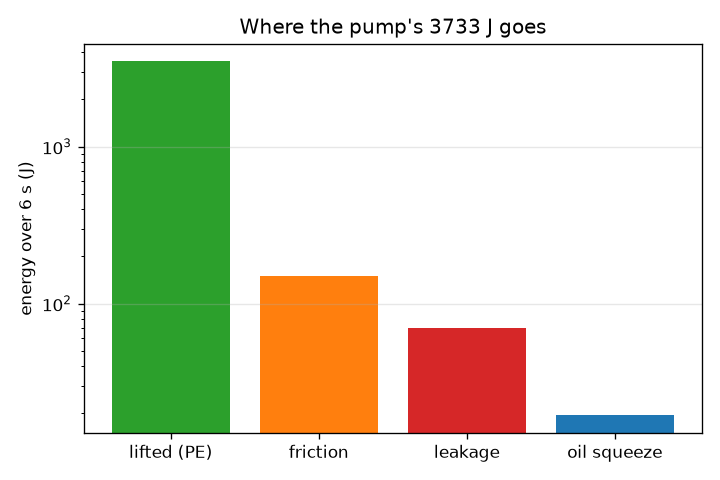
\includegraphics[width=0.85\linewidth]{figures/s03_energy_budget.png}\\\small Where the pump's energy goes in 6 s (log scale).\end{center}

\subsection*{E. Worked example}
A 1200 kg car sits on a 50 mm ram. The pump delivers 6 L/min (1e-4 m\textasciicircum{}3/s), new seals leak with c = 3e-13 m\textasciicircum{}3/(s Pa) at 40 C, seal friction is c\_f = 10 000 N s/m and the relief valve is set to 80 bar. Find the pressure the load needs, the ideal lift speed, the speed with leakage and friction, and what the 6 s simulation gives for the lift and the energy.
\begin{enumerate}[nosep]
\item Ram area A = pi * 0.050\textasciicircum{}2 / 4 = 1.9635e-3 m\textasciicircum{}2. Load pressure = m g / A = 11 772 / 1.9635e-3 = 5.996e6 Pa = 60.0 bar, below the 80 bar setting, so the relief valve stays closed.
\item Ideal speed v = Q / A = 1e-4 / 1.9635e-3 = 0.05093 m/s = 50.93 mm/s, so 6 s would give 30.6 cm.
\item Leakage flow at the load pressure: c p = 3e-13 * 5.996e6 = 1.8e-6 m\textasciicircum{}3/s, which is 1.8 percent of the pump flow.
\item Speed with leakage and friction: v = (1e-4 - 3e-13 * 11 772 / 1.9635e-3) / (1.9635e-3 + 3e-13 * 10 000 / 1.9635e-3) = 0.04997 m/s = 49.97 mm/s.
\item The simulation lifts the car 29.7 cm in 6 s (the oil first has to be squeezed to 60 bar, which costs about 0.3 cm) with a mean speed of 49.97 mm/s over the last 3 s.
\item Energy: the pump puts in 3733 J; lifted energy m g x = 3493 J (93.6 percent), friction 150 J, leakage 70 J, oil compression 19 J, kinetic 1.5 J. These add up to the input within 0.2 J.
\end{enumerate}
\textbf{Answer.} Load pressure 60.0 bar; ideal speed 50.93 mm/s; speed with leakage and friction 49.97 mm/s (the simulation agrees); lift 29.7 cm in 6 s; 93.6 percent of the 3733 J pump work becomes lifted energy and the energy budget closes within 0.2 J.

\subsection*{F. Questions}
\begin{enumerate}[nosep]
\item \textbf{Conceptual.} Why does a lift with worn seals rise more slowly when the oil is hot than when it is cold, even though the pump has not changed?
\item \textbf{Numerical.} A 1800 kg load stands on the 50 mm ram. What pressure does it need? Can a relief valve set to 70 bar let the lift work? What is the plateau pressure of that valve with the 6 L/min pump (k\_r = Q / (0.1 p\_set), c = 3e-13)?
\item \textbf{Graph and simulation interpretation.} In the left graph, the worn-seal curve at 80 C is a straight line at a lower slope. What is that slope in cm/s, and what would the slope of the ideal line be?
\item \textbf{Design and optimisation challenge.} Design: with worn seals (wear 10) and hot oil (80 C), choose a pump flow in whole L/min so that the 1200 kg car still rises at least 25 cm in 6 s, with the relief valve at 80 bar. Which flow works and what does it cost in hydraulic power p Q?
\end{enumerate}

\section{Real-world mini-project}
\textbf{Choose the cylinder and pump for a garage lift (educational).} A small garage wants a lift for cars up to 1500 kg. The relief valve is fixed at 100 bar. Choose a ram diameter from 40, 50, 63 and 80 mm and a pump flow from 3, 6, 9, 12 and 15 L/min. A design passes if (1) with new seals at 40 C the average lift speed between 4 s and 8 s is 4.0 to 6.0 cm/s, (2) with worn seals and hot oil (\texttt{wear=5.0}, \texttt{T=80.0}) it is still at least 2.5 cm/s, and (3) the pressure peak stays below 100 bar so the relief valve never opens. Use \texttt{simulate(mass=1500.0, d=..., Q=..., p\_relief=1.0e7, t\_end=8.0)} and \texttt{mean\_speed(s, 4.0)} from Session 3. Among the passing designs prefer the smallest pump flow. This is an educational exercise only: a real lift needs certified design, check valves, hoses rated for the pressure and mechanical safety locks.

\section{The path ahead}
\begin{enumerate}[nosep]
\item \textbf{Session 4: Pump strokes with check valves.} A stroke-by-stroke model of the jack with a suction and a delivery valve, replacing the continuous pump flow.
\item \textbf{Session 5: Air in the oil.} A pump model with a dead volume between the valves that is squeezed on every stroke.
\item \textbf{Session 6: Cylinder wall and pressure rating.} A small calculator that gives wall thickness from pressure, bore and allowable stress.
\item \textbf{Session 7: Controlled lowering with an orifice.} A lowering simulation with a throttle valve and a chosen opening.
\end{enumerate}

\section{Answers and hints}

\subsection*{Session 1}
\begin{enumerate}[nosep]
\item \textbf{Conceptual.} Hint: Compare force times distance on the two sides. Solution: No. The big piston moves nine times less than the small one, so the work is the same: 200 N * 0.05 m = 10 J in, and 1800 N * 0.00556 m = 10 J out. The jack trades distance for force; it does not create energy. In a real jack friction and leakage make the work out a little smaller than the work in.
\item \textbf{Numerical.} Hint: Convert 2.5 cm to 0.025 m and use A = pi d\textasciicircum{}2 / 4 and p = F / A. The multiplier is (d2 / d1)\textasciicircum{}2. Solution: A1 = pi * 0.025\textasciicircum{}2 / 4 = 4.909e-4 m\textasciicircum{}2, so p = 300 / 4.909e-4 = 611 155 Pa = 611.2 kPa. Multiplier = (10 / 2.5)\textasciicircum{}2 = 16, so F2 = 16 * 300 = 4800 N. Sanity check: the big piston is four times wider, so its area is sixteen times larger and so is the force.
\item \textbf{Graph and simulation interpretation.} Hint: Read where the curve crosses the dashed line, or solve 200 (d2 / 2)\textasciicircum{}2 = 11 772. Solution: The curve crosses the dashed line near d2 = 15.3 cm: d2 = 2 cm * sqrt(11 772 / 200) = 15.3 cm. Doubling the diameter makes the force four times bigger, which is why the curve bends upward as a parabola rather than rising in a straight line.
\item \textbf{Design and optimisation challenge.} Hint: The smallest diameter satisfies F2 = 4905 N. Then use s2 = s1 / multiplier. Solution: The smallest diameter is d2 = 1.5 cm * sqrt(4905 / 150) = 8.58 cm, so choose 9 cm. Then the multiplier is 36 and F2 = 5400 N, a margin of 10 percent. To raise the load 1 cm the pump piston must move 36 cm in total, for example six strokes of 6 cm. Trade-off: a wider big piston carries more load but needs more pumping per centimetre of lift.
\end{enumerate}

\subsection*{Session 2}
\begin{enumerate}[nosep]
\item \textbf{Conceptual.} Hint: Compare rho g h for 0.5 m of oil with the jack pressure of about 6 MPa, and with 10 m of water. Solution: The oil column in a jack is about 0.5 m tall, so rho g h = 870 * 9.81 * 0.5 = 4.27 kPa, less than 0.1 percent of the 6.37 MPa made by the pistons. A dam or diving bell has tens of metres of water: at 10 m rho g h = 98.1 kPa, about one atmosphere, and it keeps growing with depth, so it dominates the design.
\item \textbf{Numerical.} Hint: Gauge pressure is rho g h; add 101 325 Pa for the absolute pressure. Solution: Gauge pressure = 1000 * 9.81 * 30 = 294 300 Pa = 294.3 kPa = 2.94 bar. Absolute pressure = 294 300 + 101 325 = 395 625 Pa = 395.6 kPa = 3.96 bar. Sanity check: every 10 m of water adds about 1 bar.
\item \textbf{Graph and simulation interpretation.} Hint: MA = (60 / 20)\textasciicircum{}2. Lift per stroke = stroke / MA. Solution: MA = 9, F2 = 9 * 2000 = 18 000 N, which is more than 11 772 N, so it lifts the car easily. Lift per stroke = 40 / 9 = 4.44 mm, so pumps per cm = 10 / 4.44 = 2.25. Compared with the 50 mm choice (1.56 pumps per cm) the extra force margin costs about 44 percent more pumping.
\item \textbf{Design and optimisation challenge.} Hint: F1 = 8 * 150 = 1200 N. Use d2 = d1 sqrt(m g / F1) for the minimum. Solution: W = 1500 * 9.81 = 14 715 N. Minimum d2 = 16 * sqrt(14 715 / 1200) = 56.0 mm, so 60 mm works: MA = 14.06 and F2 = 16 875 N (15 percent margin). Pressure = 1200 / (pi * 0.016\textasciicircum{}2 / 4) = 5.97 MPa = 59.7 bar. Lift per stroke = 30 / 14.06 = 2.13 mm, so 4.69 pumps per cm, and the handle moves 240 mm per stroke. Trade-off: a wider ram gives more margin but more strokes; a longer lever would cut the number of strokes needed for a given force but makes the handle longer.
\end{enumerate}

\subsection*{Session 3}
\begin{enumerate}[nosep]
\item \textbf{Conceptual.} Hint: Think about viscosity and the flow past the seals. Solution: Hot oil is thinner (its viscosity is lower), so it flows more easily past worn seals: the leakage coefficient c grows with temperature. Part of the constant pump flow Q now leaks instead of moving the ram, so v = (Q - c m g / A) / (...) falls. For new seals the leakage is only about 2 percent of Q and the effect is small; for worn seals at 80 C it takes more than half of the flow.
\item \textbf{Numerical.} Hint: p = m g / A. The plateau is p = (Q + k\_r p\_set) / (c + k\_r). Solution: p = 1800 * 9.81 / 1.9635e-3 = 8.99e6 Pa = 89.9 bar, above 70 bar, so the load cannot be lifted. k\_r = 1e-4 / (0.1 * 7e6) = 1.43e-10 m\textasciicircum{}3/(s Pa), so p\_plateau = (1e-4 + 1.43e-10 * 7e6) / (3e-13 + 1.43e-10) = 76.8 bar. The pump pushes oil over the valve at 76.8 bar, which is below the 89.9 bar needed, so the ram does not move. The valve protects the system; it does not lift the car.
\item \textbf{Graph and simulation interpretation.} Hint: Slope = lift speed. Use the formula v = (Q - c m g / A) / (A + c c\_f / A) with c = 1.07e-11 m\textasciicircum{}3/(s Pa), or read the end of the curve. Solution: The ideal slope is Q / A = 5.09 cm/s. For the worn seal at 80 C, c = 3e-13 * 10 * exp(0.0318 * 40) = 1.07e-11, so the leak flow c m g / A = 6.4e-5 m\textasciicircum{}3/s, which is 64 percent of Q, and v = 1.78 cm/s (simulated: 10.5 cm in 6 s, with the first 0.3 s spent squeezing the oil). The curve is a straight line because the speed is steady once the pressure has settled to the load pressure.
\item \textbf{Design and optimisation challenge.} Hint: Try Q values with \texttt{lift\_after(wear=10.0, T=80.0, Q=...)}; the required mean speed is about 4.2 cm/s. Solution: The simulation gives 20.3 cm at 8 L/min, 25.3 cm at 9 L/min and 30.2 cm at 10 L/min; so 9 L/min is the smallest whole-number flow that meets the 25 cm target (a 1 percent margin; 10 L/min gives a bigger one). The pressure peak is 73.6 bar, below the relief setting. Hydraulic power p Q = 6.0e6 Pa * 1.5e-4 m\textasciicircum{}3/s = 900 W at 9 L/min, against 600 W for the normal 6 L/min, so the price of tolerating worn seals is a pump that is 50 percent bigger and a motor that draws more power. Replacing the seals is cheaper.
\end{enumerate}

\section{How to join}
Read \texttt{CONTRIBUTING.md} in the repository, then pick an issue labelled \texttt{good first issue}. Repository: \url{https://github.com/KrunalPanchal1995/openhydraulics}

\end{document}
